\clearpage

\section{Data/MC Comparison: Preselection Region}
\label{sec:appendix_datamc}
Here we compare data and MC distributions for data passing the 
preselection requirements. The high \pt\ dilepton trigger
data is used.

The meaning of most of the variables plotted in 
the following figures should be obvious.  There
are some exceptions that we exlain below:

All MC samples are scaled by an overall factor 1.12,
the ratio of the observed data yield in the preselection region to the
prediction from MC.
For illustration purposes, we overlay the distributions from the LM1
SUSY benchmakr point.

\begin{itemize}

\item $MT2$ is a kinematical quantity 
built from the two leptons and the \met.  For events with
two $W \to \ell$ decays it should have a sharp kinematical cutoff
at $W$ mass.  For more details, see Reference~\cite{ref:MT2}.

\item $MT2J$ is very much like $MT2$ but it is built 
out of the leptons, the \met\ and the two jets.  For $t\bar{t}$
events it has a kinematical cutoff at $M_{\rm top}$, with tails
due to the fact that occasionally one of the $b$-jets is not
found and is replaced by a gluon jet from ISR or FSR.
For more details, see Reference~\cite{ref:MT2J}.

%\item The reconstructed top mass in Figure C6 is from the 
%kinematical mass reconstruction of the top dilepton group.
%In this case we are using the $D0$ matrix-element technique.
%See Reference~\cite{ref:brown} for more details.

\end{itemize}


\clearpage

%\includepdf[pages=-, landscape=true, turn=false, offset=0mm -20mm]{datamc_ossusy.pdf}
%\includepdf[pages=-, landscape=true, turn=false, offset=0mm -20mm]{datamc_ossusy_oct15.pdf}

%Removed several plots temporarily (3rd and 4th jet pt, eta, btag info, mt)
%\includepdf[pages=-, landscape=true, turn=false, offset=0mm -20mm]{datamc_35pb.pdf}
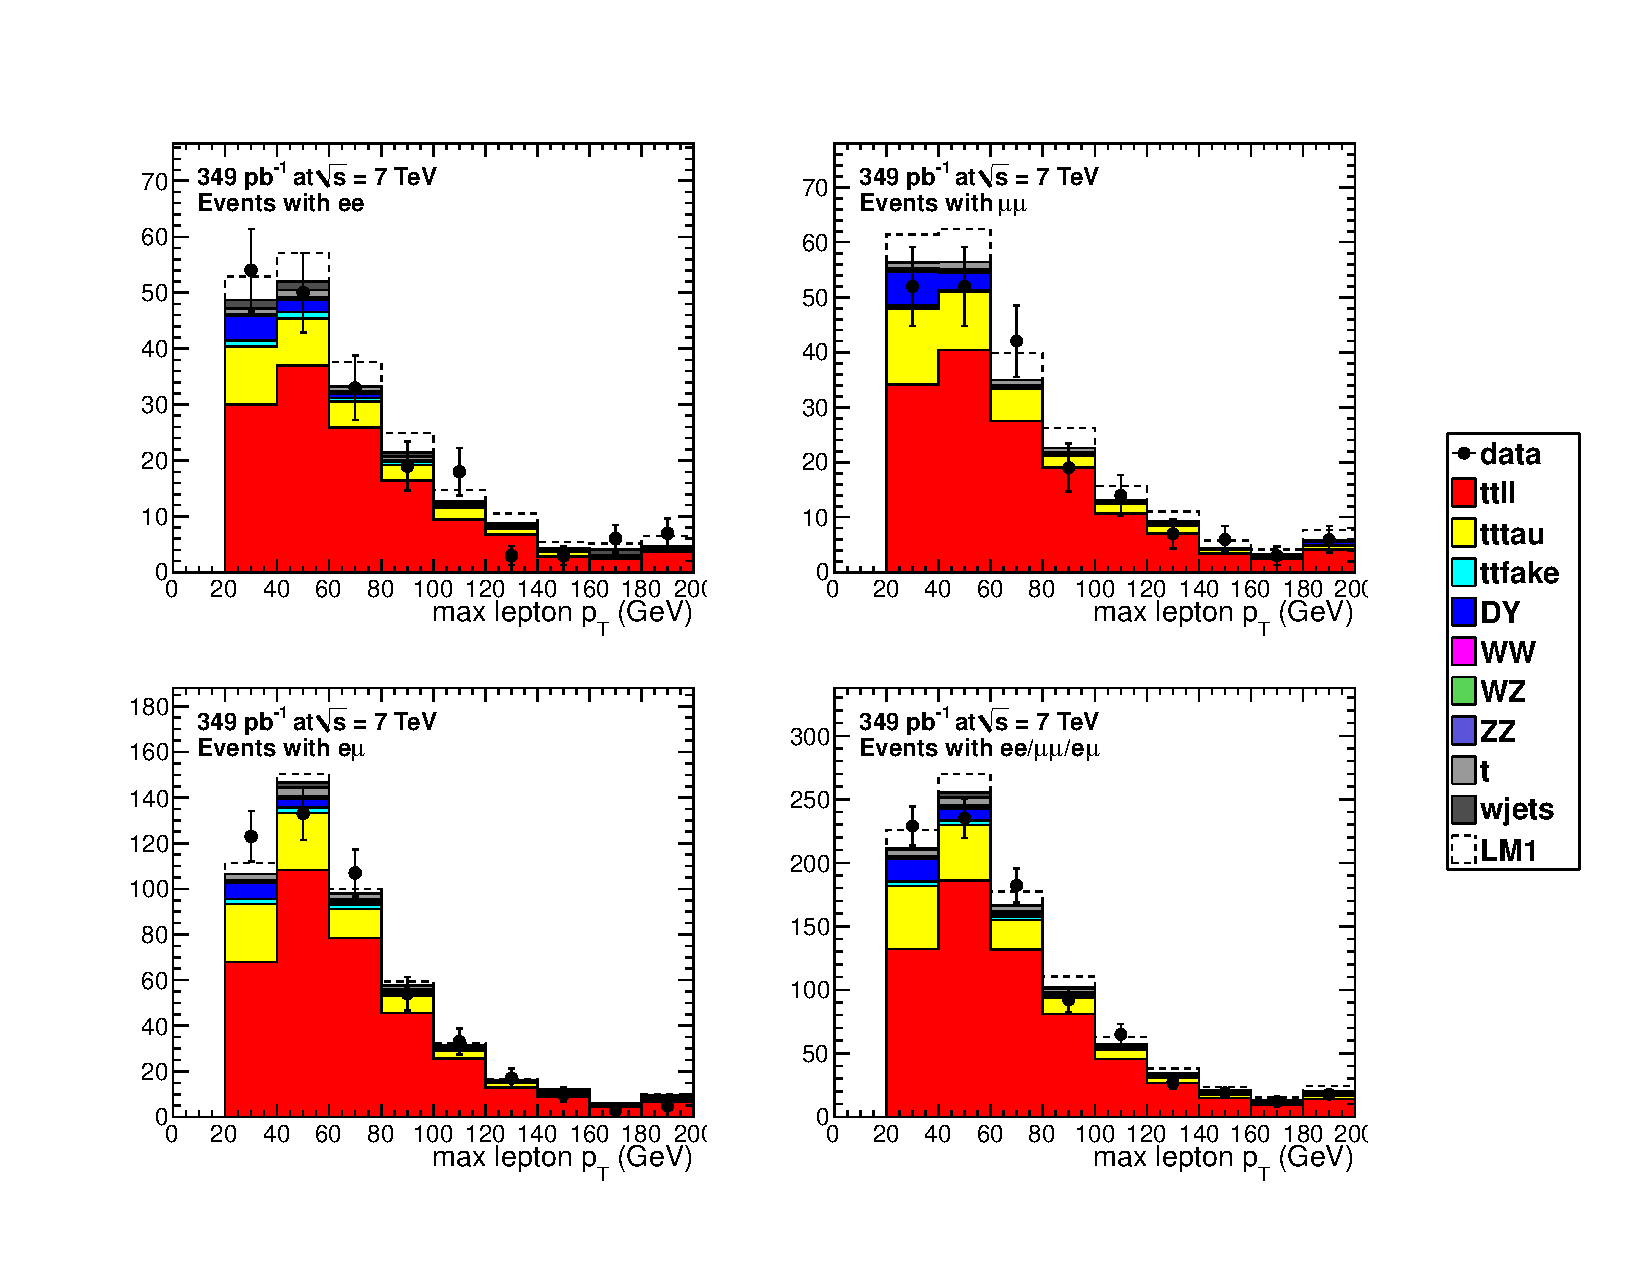
\includepdf[pages=-, landscape=true, turn=false, offset=20mm -20mm]{plots/datamc_highpt_349pb.pdf}
